\chapter{Introduction}

\emph{Contents of Chapter I, typically the introduction}

If you need help with writing \LaTeX{} code, refer to the GitLab project
\href{https://gitlab.com/davidwoodburn/latex-primer}{\LaTeX{} Primer} by David
Woodburn. Please also note the ``User Guide.pdf'' file included in this template.

The next page includes some example figures: Fig.~\ref{fig:hist} and
Fig.~\ref{fig:spec}.

Here is a citation: \textcite{savage2000} has some good information.

\begin{figure}
    \centering
    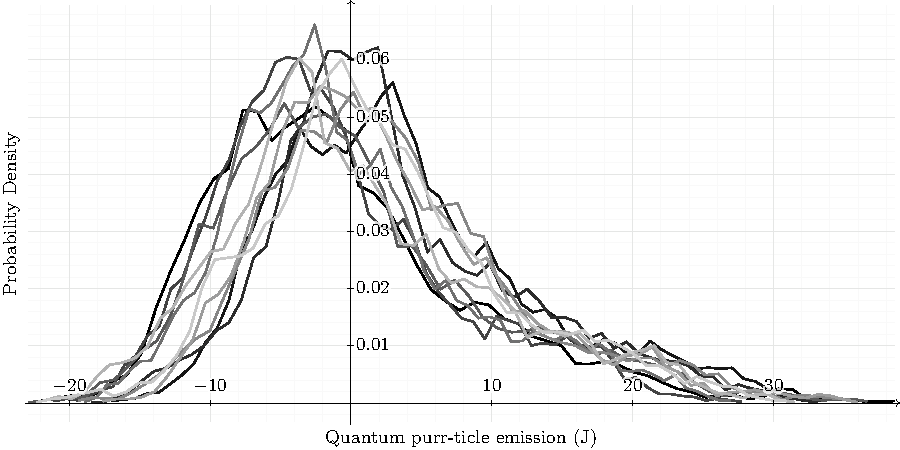
\includegraphics{fig_hist.pdf}
    \caption{Histogram of the emission energy for each of the data collects.}
    \label{fig:hist}
\end{figure}

\begin{figure}
    \centering
    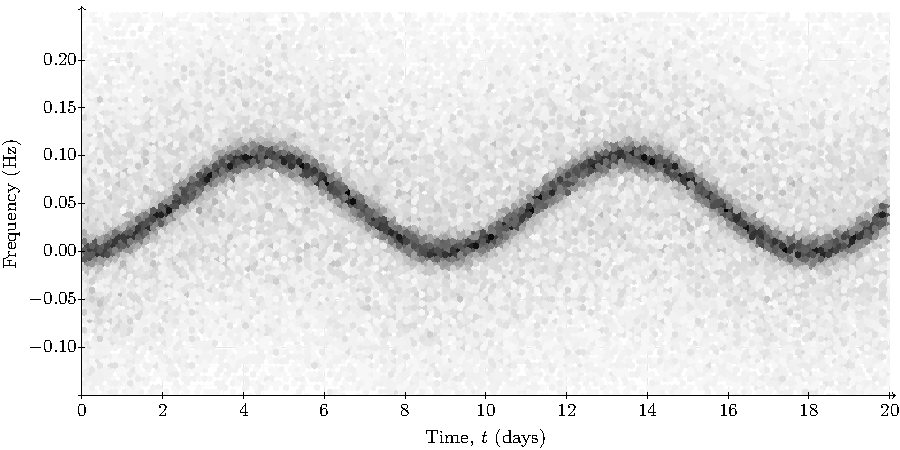
\includegraphics{fig_spec.pdf}
    \caption{Spectrogram of the emission energy over the 20-day period.}
    \label{fig:spec}
\end{figure}